\documentclass{gdl}

% CHANGE THESE
\def\groupid{BEK}
\def\projectid{AP-GCN}

\usepackage{subcaption}
\usepackage{float}

\DeclareMathOperator*{\argmin}{arg\,min}

\graphicspath{{figures/}}

\begin{document}

% CHANGE THIS
\title{AP-GCN Revisited: Replication and Alternative Approaches for Adaptive Propagation in Graph Neural Networks}

% CHANGE THIS
\author{%
Jonatan Bella, Tobias Erbacher, Jonas Knupp\\
\texttt{\{jonatan.bella, tobias.erbacher, jonas.knupp\}@usi.ch}
}

\begin{abstract}
\textcolor{red}{Concise and self-contained description of your project, motivation and main findings.}

% Delete the following part before submitting the report
\begin{center}
    \sf\large\color{red} GENERAL NOTES
\end{center}

\textcolor{red}{The report should be written as an article intended to present the findings of your work. Your aim should be to be clear and objective, substantiating your claims with references or empirical/theoretical evidence.
We are well aware of the fact that carrying out machine learning experiments might be difficult and that often the final performance might be disappointing. For this reason, you will not be evaluated solely on quantitative aspect of your work, but mainly on the quality of your analysis and report.
The length of the report should be between 4 and 8 pages (without considering references).}

\end{abstract}

\maketitle

\section{Introduction}

\textcolor{red}{Here you should clarify the context of your project and the problem you are dealing with. You should also make a brief summary of the main results and contributions (i.e., if you tried to replicate the results of an existing paper you should say if you were successful or not). The introduction should help the reader to follow along for the rest of the paper.}

This work is a replication study of the paper "Adaptive Propagation Graph Convolutional Network" by Spinelli et al. \cite{spinelli2021}. In Graph Convolutional Networks (GCNs), each node updates its representation by aggregating and transforming features from its neighbors. This process is repeated over several message passing steps, allowing nodes to incorporate information from increasingly distant parts of the graph. The core contribution of Spinelli et al. is the introduction of the Adaptive Propagation Graph Convolutional Network (AP-GCN) that allows each node in the graph to undergo an individual number of message passing steps. The number of message passing steps per node is learned during training.

In addition to the replication work, we implemented four different model architectures for allowing an individual number of message passing steps per node. We evaluated these model architectures in the same setting as AP-GCN.

[Very briefly mention/explain these approaches and tell how results are in comparison with Spinelli]. 

Our code is available on GitHub\footnote{\url{https://github.com/TobiasErbacher/gdl}}.

\section{Related works}

\textcolor{red}{Give a brief summary of (some) existing methods that are related to you project. For instance, you can refer to~\citet{gilmer2017neural}, or simply~\cite{gilmer2017neural}, for introducing Message Passing Neural Networks. In this section it is important to provide readers references to the current state of the art and the foundations of the presented method. 
N.B.: When referencing a different approach, it is not necessary to provide a detailed description, only one/two brief sentences are enough. The interested readers can eventually read the referenced work. }


The main contribution of Spinelli et al. is the introduction of the Adaptive Propagation Graph Convolutional Network (AP-GCN) which enables each node to have an individual number of message passing steps. While Spinelli et al. claim that AP-GCN was at the time the only model in which the number of message passing steps is determined independently for each node and dynamically adjusted during training, there exist model architectures that achieve a similar or at least related goal.

Xu et al. \cite{xu2018} introduced Jumping Knowledge Networks which perform a fixed number of message passes for all nodes and then use per-node LSTM attention to calculate the weighted average over the hidden vectors of the message passing rounds.   

Liu et al. \cite{liu2019} presented GeniePath networks which not only use an attention mechanism to weight the contribution of neighboring nodes but also rely on an LSTM-like gating mechanism that controls the flow of information from one message passing step to the next. In principle, GeniePath networks can learn to stop propagating information individually for each node.

Lai et al. \cite{lai2020} presented Policy-GNN which consists of two modules: a meta-policy module that relies on Deep Q-Learning predicts the required number of message passing steps per node and a GNN module that uses the meta-policy to learn graph representations.

Banino et al. \cite{banino2021} proposed the PonderNet architecture, which dynamically adjusts its computational effort based on the complexity of the given problem. While the authors do not explicitly discuss PonderNet in the context of GNNs, the architecture itself is adaptable to various neural network designs.

Xiao et al. \cite{xiao2021} presented the Learning to Propagate (L2P) framework. They use a latent discrete variable for each node that represents its optimal number of message passing steps. These variables are learned using variational Expectation-Maximization.

Finkelshtein et al. \cite{finkelshtein2024} introduced Cooperative Graph Neural Networks (Co-GNNs) where nodes are in one of the states Standard, Listen, Broadcast, or Isolate. The message-passing behavior of each node is governed by its current state. Nodes in the Broadcast state do not receive any messages but can still send messages — a situation similar to the halting mechanism in AP-GCN.

\section{Methodology}

\textcolor{red}{
\textit{You can change the name of this section as you see fit.}\\
In this section you should give a description of the methodological aspects of your work, for instance how you modified an existing method to perform a particular task or to overcome a particular limitation. If your project is about reproducibility, here you should describe the method presented in the original paper.}

In this section we first introduce the problem of having an individual number of message passing steps per node. Then, we describe the AP-GCN by Spinelli et al. Lastly, we introduce alternative architectures that allow each node to dynamically adjust its number of message passing steps. In accordance with the AP-GCN, We designed all variants to always do at least one step of message passing per node.

In traditional message-passing graph neural networks, the number of propagation steps is identical for all nodes in the graph. This uniformity implies that each node aggregates information from its neighbors through a fixed number of iterations, regardless of its individual characteristics or position within the graph structure. Spinelli et al. focus on the case where the message-passing is implemented by a Graph Convolution Network (GCN) \cite{kipf2017}. The embedding for node $\mathbf{z}_i$ after $k$ message passing iterations is

$$
\mathbf{z}_i^{k} = \sum_{j \in \mathcal{N}(i) \cup \{i\}} \frac{1}{\sqrt{\deg(i)} \cdot \sqrt{\deg(j)}} \left( \mathbf{W}^\top \cdot \mathbf{z}_j^{k-1} \right) + \mathbf{b}
$$

\subsection{AP-GCN}
The proposed Adaptive Propagation GCN (AP-GCN) enables each node in the graph to perform a distinct number of message-passing iterations, with the number being learned during training rather than set in advance. AP-GCN is inspired by the adaptive computation time in RNNs \cite{graves2017}.

A classifier is added to each node that predicts based on the hidden embedding of a node after $k$ message passing steps whether the propagation should stop. That is, the classifier predicts whether a node should stop aggregating information from its neighbors after $k$ message passing steps. The output of the classifier, $h^k_i$, is the probability the propagation should stop for node $i$ after having performed $k$ steps of message passing.

$$h^k_i = \sigma(\textbf{Q}\textbf{z}^k_i + q)$$

\noindent $\textbf{Q}$ and $q$ are trainable parameters and are shared between all nodes. There are two ways the propagation can stop. Firstly, the propagation stops if the number of propagations reaches a predefined maximum number of allowed steps $T$. Secondly, the propagation stops when the propagation budget has been used up. The budget is defined as $1-\epsilon$ where $\epsilon$ is a hyperparameter set to a small value. When $k=K_i$ the budget for node $i$ has been reached after $k$ iterations and the propagation stops. 

\begin{equation}
K_i = \min\{ k \le T \mid a_i^k = 1 \},
\end{equation}

\noindent According to Spinelli et al. the halting probabilities can be combined as

\begin{equation}
    p_i^k = 
    \begin{cases}
    R_i = 1 - \sum_{k=1}^{K_i - 1} h_i^k & \text{if } k = K_i \text{ or } k = T \\
    \sum_{l=1}^{k} h_i^l & \text{otherwise}
    \end{cases}
    \label{eq:p}
\end{equation}

\noindent so that the sequence $\{p_i\}$ forms a \textbf{cumulative probability distribution} (CDF) for the halting probabilities $\{h_i\}$. However, the sequence $\{p_i\}$ does not constitute a CDF, because for $\{p_i\}$ to be a valid CDF, it must satisfy the condition $p_i^k = 1$ when $k = K_i$ or $k = T$. This requirement arises from the fact that a CDF must converge to 1 at its maximum value, reflecting the total probability mass. Clearly, the definition by Spinelli et al., in general, violates that constraint. It could be that the error arose because AP-GCN is inspired by Graves \cite{graves2017} where in equation 6, Graves defines the $\{p_t\}$ to form a \textbf{probability mass function} (PMF) for the $\{h_t\}$ in a similar way. We did not address this issue in the replication code. In the original of \autoref{eq:p} by Spinelli et al. (equation 8) there is a second mistake: they let the sum go from $k=1$ to $K_i$ in the otherwise branch. However, this is just a typo in the paper, in the code they do it as we describe it in \autoref{eq:p}.
The output of the AP-GCN message passing layer for node $i$ is $\hat{\bf{z}}_i$ which is defined as

\begin{equation}
\hat{\mathbf{z}}_i = \frac{1}{K_i} \sum_{k=1}^{K_i} p_i^k \mathbf{z}^k_i + (1-p^k_i) \mathbf{z}_i^{k-1} 
\label{eq:aggregate}
\end{equation}

\noindent Although Spinelli et al. do not state it, this way of accumulating the contribution of the embeddings from the different propagation steps likely is inspired by the soft-conditional output from Scardapane et al. \cite{scardapane2020}.

 The propagation cost $\mathcal{S}_i$ for node $i$ is given by the sum of $K_i$ and $R_i$. Adding $\mathcal{S}_i$ to the loss term incentivizes the model to choose a limited number of propagation steps for node $i$. The propagation penalty $\alpha$ controls the trade-off between accuracy and compute time. A larger $\alpha$ encourages the model to restrict the number of propagation steps per node, whereas a smaller $\alpha$ allows for deeper message passing, potentially improving accuracy at the cost of increased computation. Spinelli et al. decided to update the halting unit once every five epochs. Thus, the final loss is

$$ \mathcal{\hat{L}} = \mathcal{L} + \alpha \sum_{i\in \mathcal{V}} \mathcal{S}_i $$


\subsection{RL-AP-GCN}
TODO: Explain role of exploration factor

In Graph Neural Networks, node representations tend to homogenize and converge as message passing progresses, a phenomenon known as over-smoothing. Rather than treating this as a limitation, this behavior can serve as a useful signal for an adaptive halting mechanism. Specifically, a reinforcement learning (RL) agent can observe how a node's embedding evolves across propagation steps and learn to halt when changes become minimal, ideally capturing the point of maximum expressiveness for that node. This stabilization suggests diminishing returns from additional message passing, indicating that sufficient neighborhood information has already been integrated. By relying solely on the task reward (e.g., classification accuracy), the policy network can learn to stop propagation at this convergence point, without requiring explicit regularization terms or penalties tied to the number of steps. In doing so, the halting decision becomes a function of information saturation rather than an externally imposed computational constraint.

This reinforcement learning implementation treats each node as an Actor Critic agent but policy and value networks are shared among all nodes. We first compute the initial node embeddings. Then, a loop begins where, at each step, the shared policy network (Actor) evaluates the current embedding of active nodes to output a halting probability, while a shared value network (Critic) estimates the expected future reward (baseline) from that state. A halting action is sampled (incorporating exploration noise during training), and propagation continues for non-halted nodes. Upon halting (or reaching the maximum iterations), a reward is calculated based primarily on the final classification correctness, and the system learns by back propagating a combined loss: a supervised loss for the GNN's classification output, and an RL loss comprising a policy gradient term (using the advantage calculated as actual reward minus the Critic's baseline), a value function loss for the Critic, and an entropy bonus to encourage exploration. To be more precise, I proceed to describe the corresponding operations: 

\paragraph{Halting policy.}
Let $\mathbf{z}_i^{k}\in\mathbb{R}^h$ be the embedding of node $i$ after $k$ message‑passing iterations. At every step the policy network produces the halting probability:
\begin{equation}
\pi_i^{k}=\sigma\bigl(g{\theta}(\mathbf{z}_i^{k})\bigr)
\end{equation}
where the parameters $\theta$ are shared across all nodes. In addition, exploration noise is injected by perturbing $\pi_i^{k}$ with Gaussian noise that decays exponentially with the epoch number. A Bernoulli action is sampled
\begin{equation}
a_i^{k} \sim \operatorname{Bernoulli}(\pi_i^{k}) ,
\end{equation}
with $a_i^{k}=1$ meaning \emph{halt}. Propagation for node $i$ stops at the first step such that:
\begin{equation}
K_i = \min\{ k \le T \mid a_i^k = 1 \},
\end{equation}
where $T$ is a hard cap on the number of iterations.

\paragraph{Reward and advantage.}
After halting, node $i$ receives a reward:
\begin{equation}
r_i = \mathbb{I}[\hat{y}i = y_i] - cK_i ,
\end{equation}
where $c\ge 0$ is the computation penalty coefficient - that we actually set to 0 during our experiments for the previously explained reasons. A shared value network $V_{\phi}$ provides a baseline, and the resulting advantage is
\begin{equation}
A_i = r_i - V_{\phi}(\mathbf{z}_i^{K_i}).
\end{equation}

\paragraph{Loss function.}
Denote by $\mathcal{V}$ the set of training nodes. The overall objective $\mathcal{V}$ to be minimized combines a standard supervised term (plus L2 regularization $\mathcal{L}_{\text{reg}}$ applied separately) and three reinforcement‑learning components, averaged over the training nodes:
\begin{align}
\mathcal{L} = &\left( \frac{1}{|\mathcal{V}|} \sum_{i\in\mathcal{V}} \mathcal{L}_{\text{NLL}}(y_i, \hat{y}_i) \right) + \mathcal{L}_{\text{reg}} \label{eq:supervised_loss_corr}\\
 &- \frac{1}{|\mathcal{V}|} \sum_{i\in\mathcal{V}} \log\pi_{i}^{K_i} A_i^{\text{detach}} \label{eq:policy_loss_corr}\\
 &+ \lambda_v \frac{1}{|\mathcal{V}|} \sum_{i\in\mathcal{V}} \bigl(r_i - V_{\phi}(\mathbf{z}_i^{K_i})\bigr)^2 \label{eq:value_loss_corr}\\
 &- \lambda_e \frac{1}{|\mathcal{V}|} \sum_{i\in\mathcal{V}} H(\pi_i^{K_i}) \label{eq:entropy_loss_corr}
\end{align}
with $H(p)= -\bigl[p\log p + (1-p)\log(1-p)\bigr]$ the binary entropy. Here $\mathcal{L}_{\text{NLL}}(y_i, \hat{y}_i)$ is the Negative Log-Likelihood loss for node $i$, and $\mathcal{L}_{\text{reg}}$ represents the L2 regularization term (e.g., $\frac{\lambda_{\text{reg}}}{2} \lVert\theta_{\text{reg}}\rVert^2$ applied to specific parameters $\theta_{\text{reg}}$). $A_i^{\text{detach}}$ represents the advantage $r_i - V_{\phi}(\mathbf{z}_i^{K_i})$ where the gradient is not propagated back through the value function estimate $V_{\phi}(\mathbf{z}_i^{K_i})$ during the policy update (as indicated by `detach` - to ensure stable training by preventing the policy update from interfering with the value function update, as the policy might try to manipulate the value estimates to make its own actions look better, rather than simply improving the policy based on the current value estimate.). Hyper‑parameters $\lambda_v$ (corresponding to `value\_weight` in the code) and $\lambda_e$ (corresponding to `entropy\_weight`) weight the value‑regression and entropy‑regularization terms, respectively. The signs reflect the objective minimization: the negative sign in eq.~\eqref{eq:policy_loss_corr} implements policy gradient ascent (maximizing expected rewards), and the negative sign in eq.~\eqref{eq:entropy_loss_corr} encourages entropy maximization (promoting exploration).
    
There are several extensions that could enhance the implementation. The sparse, delayed reward signal could be augmented with denser, intermediate rewards reflecting confidence gains at each step. The RL state representation could be enriched beyond the current embedding to include neighboring node embeddings difference or a history of embeddings (using RNNs or attention), giving the policy more context. Employing more advanced RL algorithms such as PPO for policy updates or GAE for advantage estimation could improve training stability and sample efficiency compared to the current REINFORCE-with-baseline approach. Finally, refining the training strategy, perhaps by alternating between supervised and RL optimization steps, could further stabilize learning and potentially improve final performance.

\subsection{Ponder-AP-GCN}
Strongly inspired by PonderNet \cite{banino2021}, we adopted its core ideas to implement a halting mechanism for GCN. We define $\lambda_i^k$ as the conditional probability that node $i$ halts after $k$ message passing steps given that node $i$ has not halted before. Then, the unconditional probability of node $i$ halting after $k$ message passing iterations is

$$
p_i^k = \lambda_i^k \prod_{j=1}^{k-1} (1-\lambda_i^j)
$$

\noindent which is similar to the geometric distribution but with variable $\lambda$. This would be a valid distribution if we integrated over all possible message passing steps, which is infeasible in practice. For this reason, we define a maximum number of propagation steps $T$ and assign all remaining probability to the last step. This ensures that the $\{p_i^k\}$ for $k\in \{1,...,T\}$ sum to 1. The embedding for node $i$ and therefore implicitly also how many message passing steps are done is then sampled from the random variable $\mathcal{Z}_i$ with probability density distribution $P(\mathcal{Z}_i=\hat{\mathbf{z}}_i^k) = p_i^k$.

The model is trained end-to-end by minimizing the loss function that consists of a sum of two terms weighted by hyperparameter $\beta$: the reconstruction loss and the regularization loss:

\begin{equation}
L = \sum_{i=1}^{\mathcal{|V|}} \sum_{k=1}^{T} \underbrace{p_i^k \mathcal{L}(y_i, \hat{y}_i^k)}_{\text{reconstruction}} + \beta \underbrace{KL(\mathbf{p}_i || p_G(\lambda_p))}_{\text{regularization}}
\label{eq:ponder-loss}
\end{equation}

\noindent where $|V|$ is the number of nodes in the graph.

\noindent The reconstruction loss per node is the cross-entropy loss averaged over the $T$ steps weighted by their corresponding halting probability $p_n$. The regularization term per node incentivizes the distribution $p_n$ to stay close to a predefined prior geometric distribution $p_G$ with parameter $\lambda_p$. In comparison to AP-GCN, this regularization term has the advantage that it is easily interpretable. In particular, setting the prior parameter $\lambda_p = \frac{1}{N}$ encourages the model towards halting after an average of $N$ steps. A disadvantage of Ponder-AP-GCN, compared to AP-GCN, is that during training it must compute the halting distribution over all $T$ steps for each node, whereas AP-GCN can stop computations as soon as a node halts. However, since all the computations in AP-GCN are implemented using matrix operations to deal with all the nodes simultaneously it is questionable whether this is an actual advantage in practice.

Focusing on our implementation, the model architecture starts with an MLP that processes the node features, followed by the recurrent GCN propagation steps - similar to the AP-GCN. A key component is the shared linear halting unit that computes logits at each step, which are passed through a sigmoid function to yield the conditional halting probabilities $\lambda_n$. The unconditional halting distribution $p_n$ is then derived iteratively from these $\lambda_n$  values, ensuring the probabilities sum to one over the maximum N steps. The training loss combines the expected loss (weighted by $p_n$) and the KL divergence between the learned $p_n$ and the geometric prior $p_G$, scaled by $\beta$. Inference can be performed either by first computing the full distribution p and selecting the step via argmax or sampling, or through the computationally efficient sequential Bernoulli sampling at each step as proposed in the PonderNet paper. We implemented the first approach and use the temperature parameter to control the randomness in the model's output. A low temperature makes the model more likely to select high-probability halting steps from $\mathbf{p}_i$, whereas a high temperature increases the likelihood of selecting lower-probability halting steps.

\subsection{Gumbel-AP-GCN}
TODO:  explain role of $\tau_{\text{initial}}$, $\tau_{\text{warmup}}$, $\tau_{\text{decay}}$, and $\tau_{\text{final}}$ 


The Gumbel-AP-GCN architecture is based on the Ponder-AP-GCN architecture but instead of calculating the loss as expectation over the halting steps as in \autoref{eq:ponder-loss}, a halting step $h_i$ for node $i$ is sampled from the learned distribution $\mathbf{p}_i$ of halting steps. We use the Gumbel-Softmax technique \cite{Maddison2017, Jang2017} to draw a sample in a differentiable way. Thus, the halting step for node $i$ is defined as

$$
    h_i = \arg\max \text{GumbelSoftmax}(\{\log p_i^1,...,\log p_i^{T}\}, \tau)
$$

\noindent where $\tau$ is the temperature parameter controlling how sharp (low $\tau$) or smooth (high $\tau$) the output distribution is. We apply temperature annealing by starting with a higher temperature to encourage exploration in the early stages of training, and gradually lowering it to produce less uniform distributions as training progresses.

Instead of computing the expected loss over all halting steps like in Ponder-AP-GCN, we compute it from the output corresponding to the sampled step:

$$
L = \sum_{i=1}^{\mathcal{|V|}} \underbrace{p_i^{h_i} \mathcal{L}(y_i, \hat{y}_i^{h_i})}_{\text{reconstruction}} + \beta \underbrace{KL(\mathbf{p}_i || p_G(\lambda_p))}_{\text{regularization}}
$$

\noindent The KL divergence hyperparameter is set to 0, so that the halting policy is learned solely by optimizing the task performance at the sampled steps without explicit regularization. 

The inference is implemented similar to the training. A halting step is sampled using the GumbelSoftmax function and the output corresponding to that halting steps is returned. As in the Ponder-AP-GCN, the inference could be implemented more efficiently using sequential Bernoulli sampling.

\subsection{Co-AP-GCN}

\section{Implementation}

\textcolor{red}{
This section should be structured as follows (from the Reproducibility challenge template):
---
Briefly describe what you did and which resources did you use. E.g. Did you use author's code, did you re-implement parts of the pipeline, how much time did it take to produce the results, what hardware you were using and how long it took to train/evaluate. }

We independently implemented AP-GCN and compared our implementation with the reference code provided by Spinelli et al., available on their GitHub repository\footnote{\url{https://github.com/spindro/AP-GCN}}. We found that in cases where nodes reach the maximum propagation limit $T$ and are eligible to propagate further, the implementation by Spinelli et al. incorrectly reports one additional step, resulting in an off-by-one error. Importantly, the implementation does not actually perform an extra propagation step—it only misreports the number of steps taken.

For the loading of the \texttt{Citeseer}, \texttt{Cora-ML}, \texttt{PubMed}, \texttt{MS-Academic}, \texttt{A. Computer}, and \texttt{A. Photo} datasets we used the code provided by Spinelli et al.

We asked Prof. Spinelli, among other questions, why they placed the feature mapping layer that projects to the number of classes before the message passing layer. However, we did not receive a response to our email.

\subsection{Datasets}
\textcolor{red}{Describe the datasets you used and how you obtained them. }

We downloaded the \texttt{Citeseer} \cite{sen2008}, \texttt{Cora-ML} \cite{mccallum2000}, \texttt{PubMed} \cite{namata2012}, \texttt{MS-Academic} \cite{shchur2018}, \texttt{A. Computer}, and \texttt{A. Photo} datasets from the GitHub repository of Spinelli et al. along with the code to load them. The \texttt{A. Computer} and \texttt{A. Photo} datasets are portions of the Amazon co-purchase graph originally presented in \cite{mcauley2015}. In the \texttt{Microsoft Academic} dataset, the edges represent co-authorship while in the \texttt{Citeseer}, \texttt{Cora-ML}, and \texttt{PubMed} datasets, the edges represent citations. All these datasets consists of a single graph and are node classification problems. Only the largest connected component in each dataset is used. The features are bag of words representations of the papers' abstracts. We calculated the statistics for each dataset, as shown in \autoref{tab:dataset_statistics}. Except for a few values in the average degrees, which may be due to rounding, our results are consistent with those reported by Spinelli et al.

\begin{table}[h]
    \small\sf
    \setlength{\tabcolsep}{2pt}
    \caption{Dataset Statistics}
    \begin{tabular}{l c c c c c c}
        \toprule
        Dataset & Classes & Features & Nodes & Edges & Avg. Degree \\
        \midrule
        Citeseer & 6 & 3703 & 2110 & 3668 & 6.95 \\
        Cora-ML & 7 & 2879 & 2810 & 7981 & 11.36 \\
        PubMed & 3 & 500 & 19717 &44324 &8.99 \\
        MS-Academic & 15&6805 & 18333 & 81894 & 17.87 \\
        A.Computer & 10 & 767 & 13381 & 245778 & 73.47 \\
        A.Photo  & 8 & 745 & 7487 & 119043 & 63.60 \\
        \bottomrule
    \end{tabular}
    \label{tab:dataset_statistics}
\end{table}

\subsection{Hyperparameters}
\textcolor{red}{Describe how you set the hyperparameters and what was the source for their value (e.g. paper, code or your guess). }

In the experiments with AP-GCN we used the hyperparameters described by Spinelli et al. They are described in appendix \ref{lab:hyper-ap-gcn}. The hyperparameters used in the experiments with RL-AP-GCN, Ponder-AP-GCN, and Gumbel-AP-GCN are available in appendices \ref{lab:hyper-rl-gcn}, \ref{lab:hyper-ponder-gcn}, and \ref{lab:hyper-gumbel-gcn}. We did not perform extensive hyperparameter optimization for RL-AP-GCN, Ponder-AP-GCN, and Gumbel-AP-GCN. In fact, we mostly tested each model on a single dataset and once we obtained reasonably good hyperparameters we reused them for the other datasets. The only exception is the weight decay, which was set to a different value for the Amazon datasets compared to the other datasets.

\subsection{Experimental setup}
\textcolor{red}{Explain how you ran your experiments, e.g. the CPU/GPU resources and provide the link to your code and notebooks.}

We follow the experimental setup of Spinelli et al., splitting each dataset into a training, a validation, and a test set. Spinelli et al. follow the experimental setup of \cite{}. The validation set is used to detect early stopping, while the test set serves to evaluate the final model performance. The union of the training and validation is considered to be the "visible" or "development" set. For the \texttt{MS-Academic} dataset, the development set consists of 5,000 samples, whereas for all other datasets it contains 1,500 samples. This larger size is chosen for \texttt{MS-Academic} because a smaller development set of 1,500 samples would likely result in fewer than 20 samples per class. For each dataset, we use 20 random seeds, and for each seed, the model is trained five times with different weight initializations, resulting in 100 trained models per dataset for a fixed set of hyperparameters.

While Spinelli et al. provided the seeds for the train/validation/test split, there is still randomness because of the model initializations. Since Spinelli et al. did not provide a seed to account for this, we selected the seed $11$ to make the model initializations reproducible. 

We report the average accuracy when using a training set of 20 nodes per class, with uncertainties showing the 95\% confidence level calculated by bootstrapping. The uncertainty is defined as the larger absolute difference between the mean and the 2.5th or 97.5th percentile of the bootstrap distribution. This follows the code in the Jupyter notebook provided by Spinelli et al. In each run we also save when each node in the test set halts.

\subsection{Computational requirements}
\textcolor{red}{Provide information on computational requirements for each of your experiments. For example, the number of CPU/GPU hours and memory requirements. You'll need to think about this ahead of time, and write your code in a way that captures this information so you can later add it to this section. }

The experiments were conducted on a MacBook Pro with Apple M2 Pro Chip and 16 GB of memory. We used the \texttt{mps} backend of PyTorch.


\section{Results}

\textcolor{red}{In this section you should report the results of your work (e.g., the outcome of an empirical analysis). You should be objective and support your statements with empirical evidence.}

\begin{table*}[h]
    \small\sf\centering
    \caption{Average test set accuracies with 95\% confidence intervals, computed from 100 runs per model using 20 random seeds and 5 different initial weight settings per seed.}
    \begin{tabular}{l c c c c c c}
        \toprule
        Model & Citeseer & Cora-ML & PubMed & MS-Academic & A.Computer & A.Photo\\
        \midrule
        \texttt{RL-AP-GCN} &$74.65 \pm 0.29$&$81.60 \pm 1.38$&$77.16 \pm 0.42$&$88.32 \pm 0.41$&$79.94 \pm 0.52$&$88.89 \pm 0.43$ \\
        \texttt{Ponder-AP-GCN} &$74.80 \pm 0.31$&$82.14 \pm 0.31$&$76.37 \pm 0.41$&$91.29 \pm 0.12$&$83.41 \pm 0.25$&$91.27 \pm 0.23$ \\
        \texttt{Gumbel-AP-GCN} &$70.09 \pm 1.25$&$70.92 \pm 2.34$&$76.83 \pm 0.49$&$87.56 \pm 0.45$&$79.13 \pm 0.58$&$89.21 \pm 0.44$ \\
        \texttt{Co-AP-GCN}  \\
        \texttt{AP-GCN replication} &$75.88 \pm 0.27$&$83.69 \pm 0.33$&$78.98 \pm 0.40$&$91.66 \pm 0.14$&$83.26 \pm 0.34$&$90.68 \pm 0.32$\\
        \midrule
        \texttt{AP-GCN} & $76.12 \pm 0.24$ & $85.71 \pm 0.22$ & $79.80 \pm 0.34$ & $92.62 \pm 0.07$ & $85.18 \pm 0.23$ & $92.05 \pm 0.22$\\
        \bottomrule
    \end{tabular}
    \label{tab:table}
\end{table*}

\textcolor{red}{Use figures, plots and tables (like \autoref{tab:table}) to present your results in a nice and readable way.}

We report the results of our experiments with the AP-GCN, Graph PonderNet, RL, and CoGNN architectures. For each model architecture we report the distribution of the halting steps, i.e., the steps at which each node halts. Since we have data from 100 runs per model architecture, we first average the halting steps for each node over the 100 runs and then plot the distribution obtained using kernel density estimation (KDE) over these averaged halting steps per node. Note that because of the averaging and the KDE there can be probability mass at non-integer values even though in reality all the models can only halt after an integer number of steps. This approach follows the methodology used by Spinelli et al.


\subsection{AP-GCN}

\subsection{RL-AP-GCN}

\subsection{Ponder-AP-GCN}

\subsection{Gumbel-AP-GCN}

\subsection{Co-AP-GCN}

\begin{figure*}[p]
    \centering
    \begin{minipage}[t]{0.48\textwidth}
        \centering
        \begin{subfigure}[b]{0.7\textwidth}
            \centering
            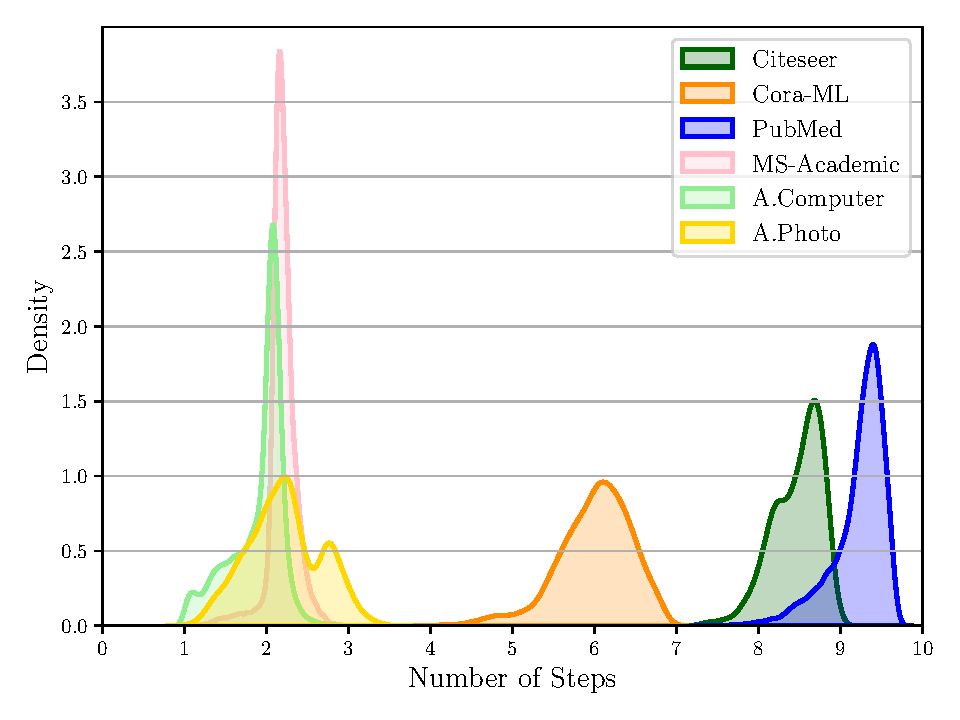
\includegraphics[width=\textwidth]{Spinelli_steps_distribution.pdf}
            \captionsetup{justification=centerlast}
            \caption{AP-GCN Replication}
            \label{fig:step_dist_AP_GCN}
        \end{subfigure}
        
        \begin{subfigure}[b]{0.7\textwidth}
            \centering
            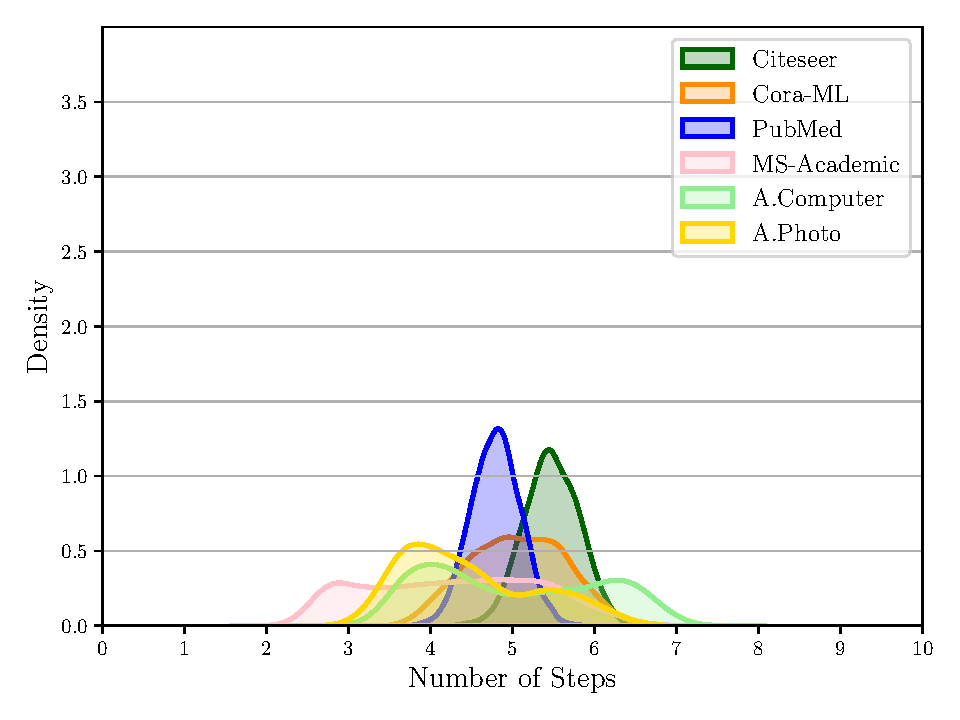
\includegraphics[width=\textwidth]{RL-AP-GCN_steps_distribution.pdf}
            \captionsetup{justification=centerlast}
            \caption{RL-AP-GCN}
            \label{fig:step_dist_RL_AP_GCN}
        \end{subfigure}
        
        \begin{subfigure}[b]{0.7\textwidth}
            \centering
            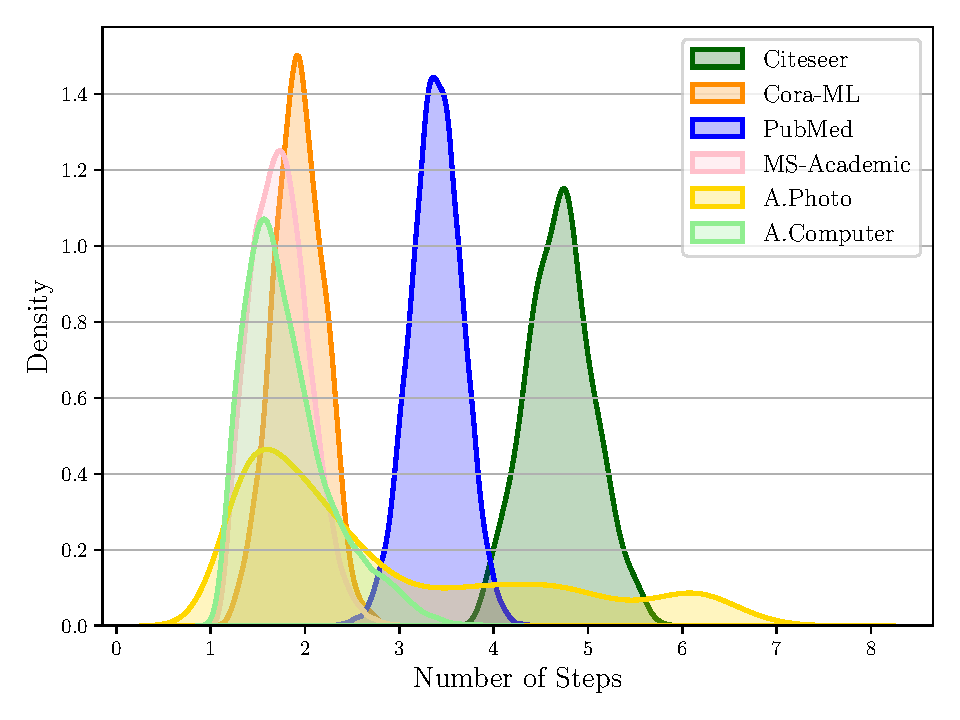
\includegraphics[width=\textwidth]{Ponder-AP-GCN_steps_distribution.pdf}
            \captionsetup{justification=centerlast}
            \caption{Ponder-AP-GCN}
            \label{fig:step_dist_Ponder_AP_GCN}
        \end{subfigure}
        
        \begin{subfigure}[b]{0.7\textwidth}
            \centering
            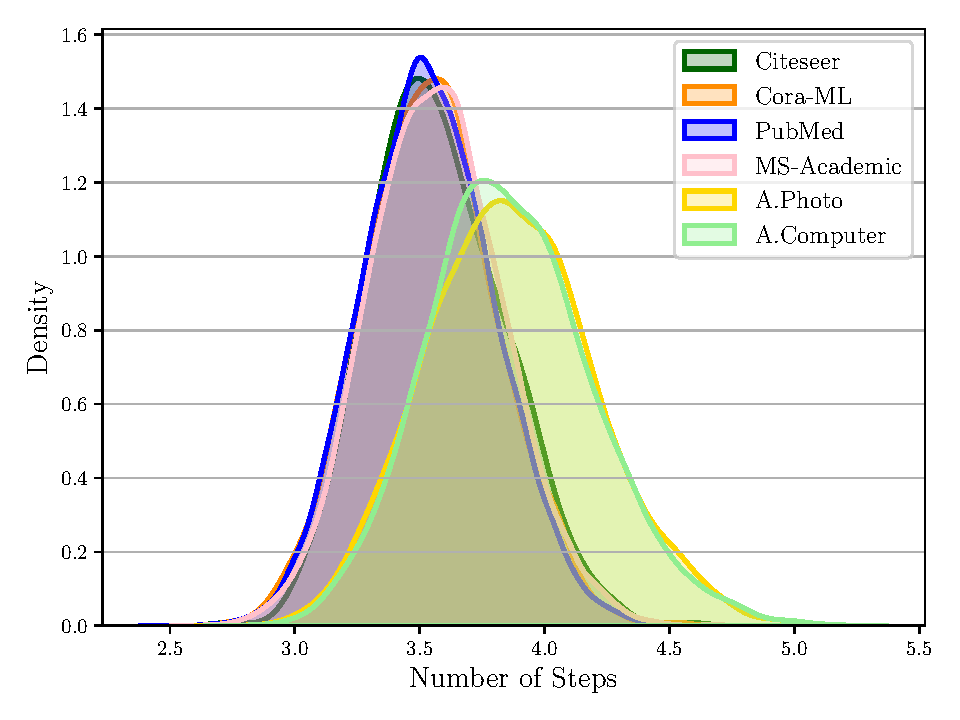
\includegraphics[width=\textwidth]{Gumbel-AP-GCN_steps_distribution.pdf}
            \captionsetup{justification=centerlast}
            \caption{Gumbel-AP-GCN}
            \label{fig:step_dist_Gumbel_AP_GCN}
        \end{subfigure}
        
        \begin{subfigure}[b]{0.7\textwidth}
            \centering
            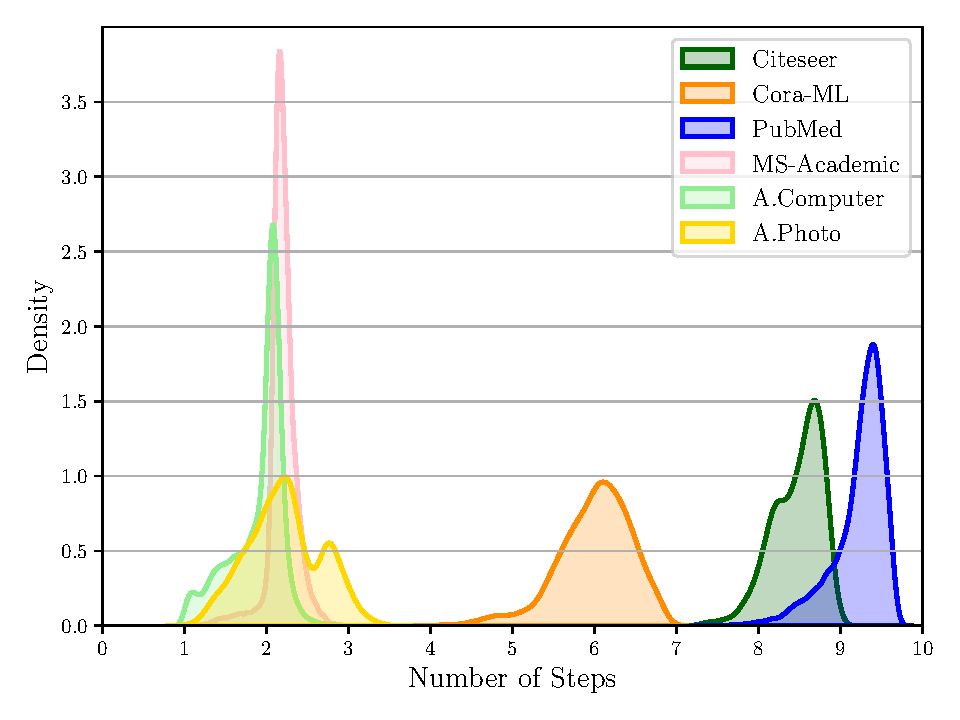
\includegraphics[width=\textwidth]{Spinelli_steps_distribution.pdf}
            \captionsetup{justification=centerlast}
            \caption{Co-AP-GCN}
            \label{fig:step_dist_Co_AP_GCN}
        \end{subfigure}
        
        \captionsetup{justification=centerlast}
        \caption{Average density distribution of the halting steps for the five different model architectures for each dataset.}
        \label{fig:main}
    \end{minipage}%
    \hfill
    \begin{minipage}[t]{0.48\textwidth}
        \centering
        \begin{subfigure}[b]{0.7\textwidth}
            \centering
            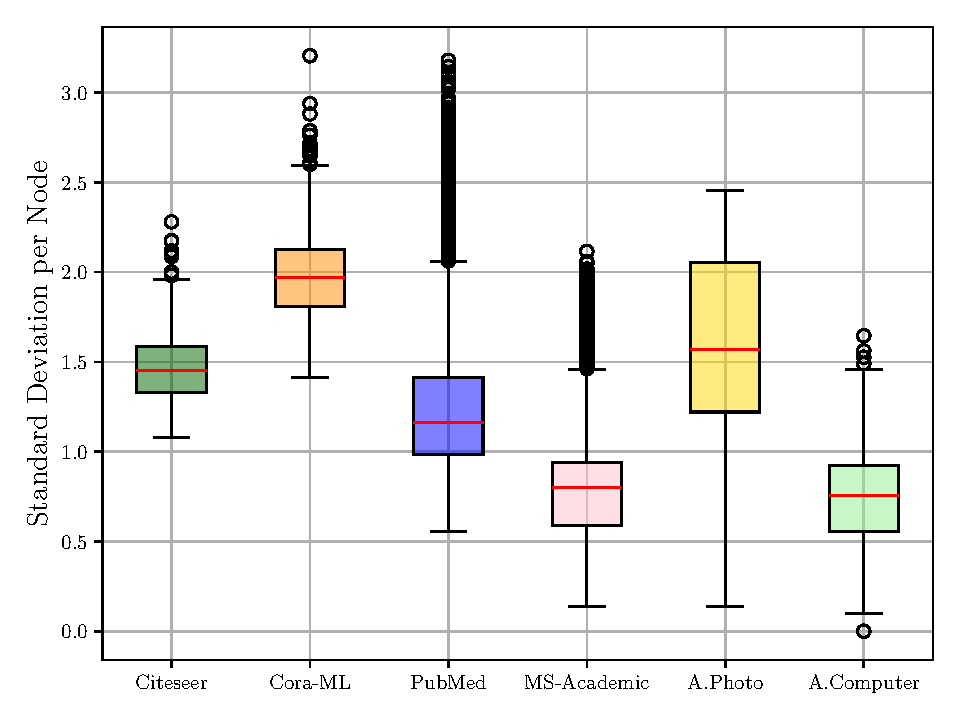
\includegraphics[width=\textwidth]{Spinelli_std_steps_per_node_boxplot.pdf}
            \captionsetup{justification=centerlast}
            \caption{AP-GCN Replication}
            \label{fig:step_std_AP_GCN}
        \end{subfigure}
        
        \begin{subfigure}[b]{0.7\textwidth}
            \centering
            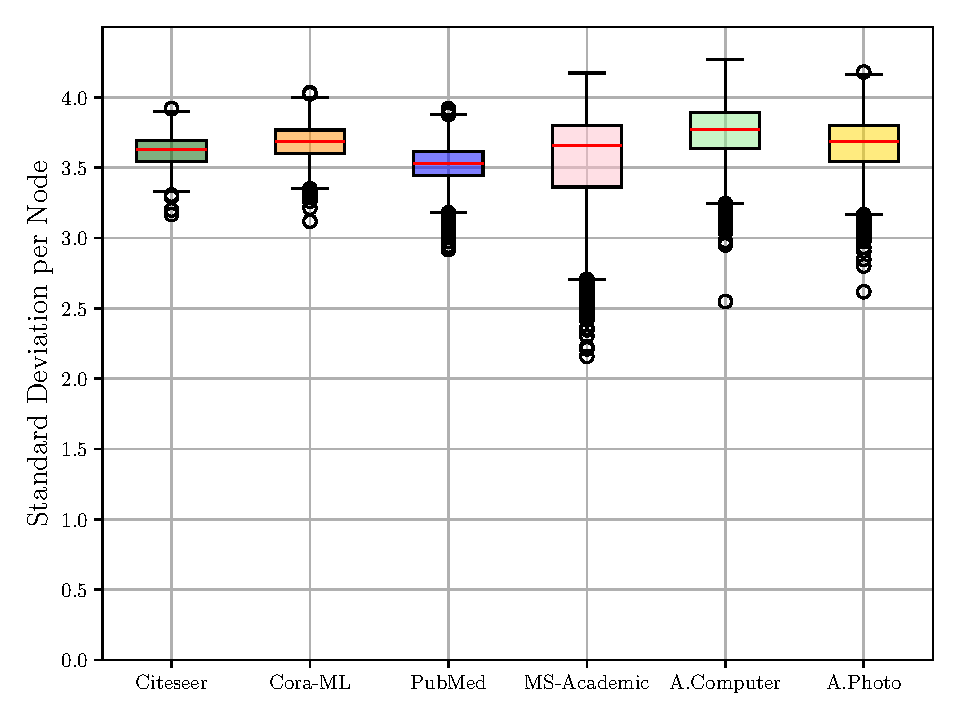
\includegraphics[width=\textwidth]{RL-AP-GCN_std_steps_per_node_boxplot.pdf}
            \captionsetup{justification=centerlast}
            \caption{RL-AP-GCN}
            \label{fig:step_std_RL_AP_GCN}
        \end{subfigure}
        
        \begin{subfigure}[b]{0.7\textwidth}
            \centering
            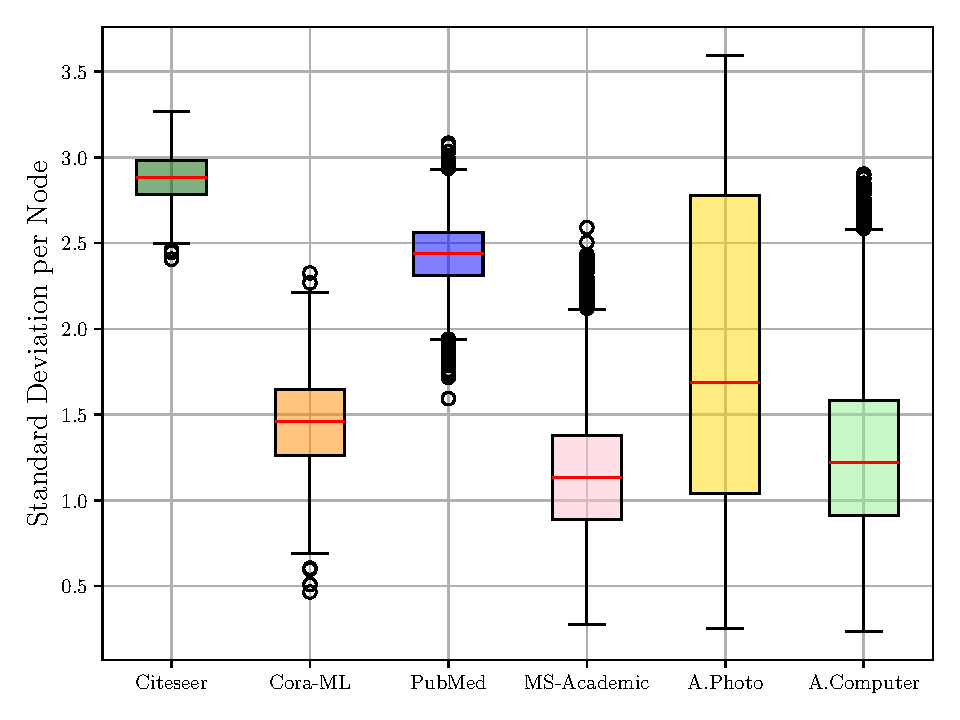
\includegraphics[width=\textwidth]{Ponder-AP-GCN_std_steps_per_node_boxplot.pdf}
            \captionsetup{justification=centerlast}
            \caption{Ponder-AP-GCN}
            \label{fig:step_std_Ponder_AP_GCN}
        \end{subfigure}
        
        \begin{subfigure}[b]{0.7\textwidth}
            \centering
            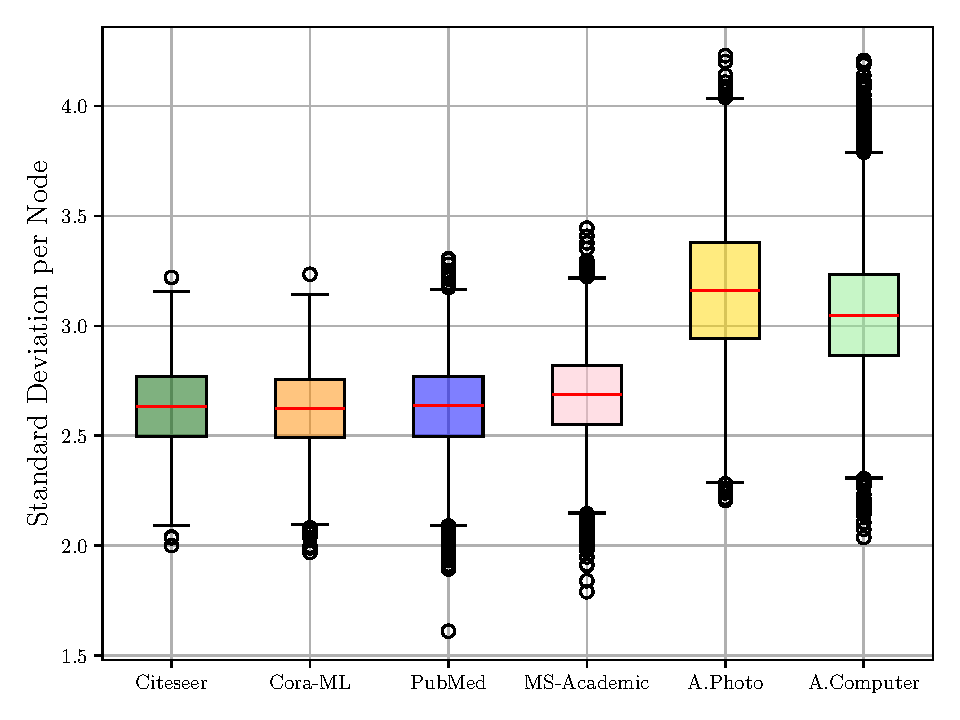
\includegraphics[width=\textwidth]{Gumbel-AP-GCN_std_steps_per_node_boxplot.pdf}
            \captionsetup{justification=centerlast}
            \caption{Gumbel-AP-GCN}
            \label{fig:step_std_Gumbel_AP_GCN}
        \end{subfigure}
        
        \begin{subfigure}[b]{0.7\textwidth}
            \centering
            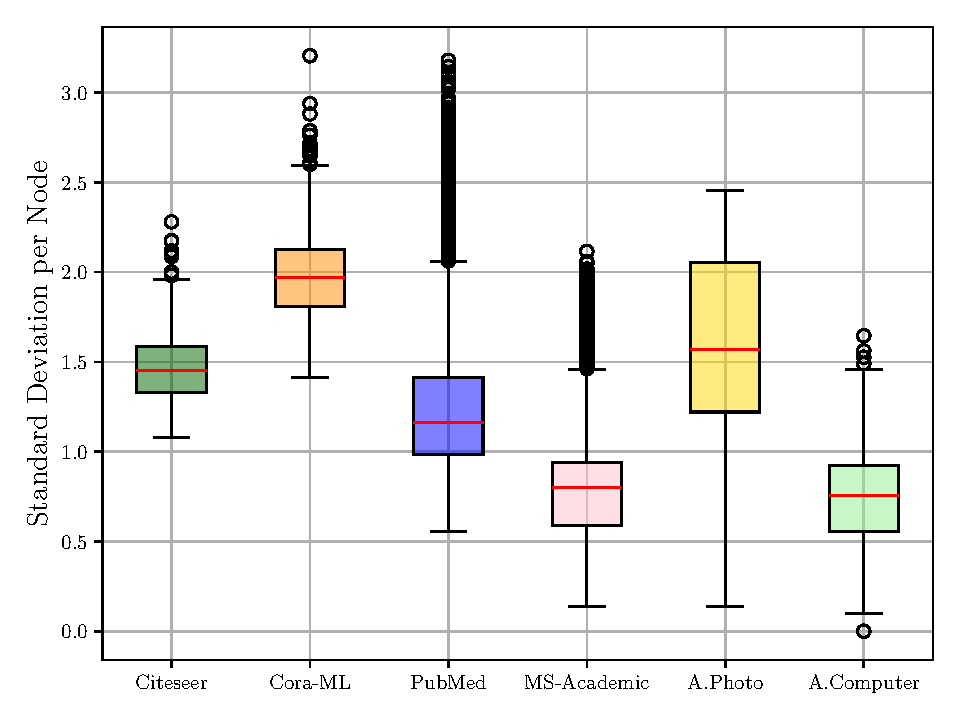
\includegraphics[width=\textwidth]{Spinelli_std_steps_per_node_boxplot.pdf}
            \captionsetup{justification=centerlast}
            \caption{Co-AP-GCN}
            \label{fig:step_std_Co_AP_GCN}
        \end{subfigure}
        
        \captionsetup{justification=centerlast}
        \caption{Standard deviations per node over the 100 experiments for each dataset.}
        \label{fig:steps_dist_steps_std}
    \end{minipage}
\end{figure*}


\section{Discussion and conclusion}

\textcolor{red}{Here you can express your judgments and draw your conclusions based on the  evidences produced on the previous sections.
Try to summarize the achievements of your project and its limits, suggesting (when appropriate) possible extensions and future works.}

While AP-GCN works well empirically, some of its choices are hard to justify from a theoretical point of view in our opinion. For instance, Spinelli et al. call $h_i^k$ the probability that a node should halt after $k$ iterations. However, this is actually not what happens, because a node halts when the propagation budget is used up or the maximum number of propagation steps is reached. For instance, assume we have $\mathbf{h}_i = [0.3, 0.4, 0.25]$ and propagation budget $0.9$. AP-GCN will not make node $i$ halt with probability $0.3$ after the first step. In fact, it will never halt after the first step. It will only halt after the third step when the propagation budget is used up. Similarly, the way the embeddings are aggregated over the steps in \autoref{eq:aggregate} has no real theoretical justification.


\clearpage
% Bibliography
\bibliography{bibliography}
\bibliographystyle{unsrtnat}
\clearpage

\appendix

\section{Hyperparameters}
The maximum number of steps $T$ was set to 10 for all experiments.

\subsection{AP-GCN}
\label{lab:hyper-ap-gcn}
We use 2 feature transformation layers, a dropout rate of 0.5, 64 hidden units, and the Adam optimizer with learning rate 0.01. We applied $L2$ regularization with coefficient 0.008 on the parameters of the first layer. For the \texttt{A. Photo} and \texttt{A. Computer} no regularization was used.

\subsection{RL-AP-GCN}
\label{lab:hyper-rl-gcn}
We used the Adam optimizer with a learning rate of 0.01. The model employs a dropout rate of 0.5 and 64 hidden units. $L_2$ regularization with a coefficient of 0.008 was applied to the parameters of the first layer, except for the \texttt{A. Photo} and \texttt{A. Computer} datasets, where no regularization was used. The entropy weight was set to 0.01, and the value weight to 0.5. Gradient norm clipping was applied across all model parameters with a maximum norm of 1.0. Additionally, we set the computation penalty to 0, used an exploration factor of 0.01, and did not employ any scheduling for the exploration penalty.

\subsection{Ponder-AP-GCN}
\label{lab:hyper-ponder-gcn}
We used the Adam optimizer with a learning rate of 0.01. The model incorporates a dropout rate of 0.5, an edge dropout rate of 0.3, and 64 hidden units. Edge dropout was applied only in the section focused on adaptive message propagation. $L_2$ regularization with a coefficient of 0.008 was applied to the parameters of the first layer, except for the \texttt{A. Photo} and \texttt{A. Computer} datasets, where no regularization was used. We set $\beta$ to 0.01 and $\lambda_p$ to 0.2. During inference, a temperature value of 5.0 was used.

\subsection{Gumbel-AP-GCN}
\label{lab:hyper-gumbel-gcn}
We employed the Adam optimizer with a learning rate of 0.01. The model uses a dropout rate of 0.5, an edge dropout rate of 0.3, and 64 hidden units. Edge dropout was applied exclusively in the adaptive message propagation component. $L_2$ regularization with a coefficient of 0.008 was applied to the parameters of the first layer, except for the \texttt{A. Photo} and \texttt{A. Computer} datasets, where no regularization was used. We set $\beta$ to 0, indicating that the model learns without a geometric prior, rendering $\lambda_p$ irrelevant. During training we use a scheduler for $\tau$ with $\tau_{\text{initial}} = 10.0$, $\tau_{\text{warmup}} = 20.0$, $\tau_{\text{decay}} = 50.0$, and $\tau_{\text{final}} = 1.0$. During evaluation, $\tau$ was fixed at 0.01.

\end{document}
